% This is samplepaper.tex, a sample chapter demonstrating the
% LLNCS macro package for Springer Computer Science proceedings;
% Version 2.21 of 2022/01/12
%
\documentclass[runningheads]{llncs}
\usepackage{enumitem}
\setlist[enumerate,1]{label={\arabic*.}}
\setlist[enumerate,2]{label={\alph*.}}
%
\usepackage[T1]{fontenc}
% T1 fonts will be used to generate the final print and online PDFs,
% so please use T1 fonts in your manuscript whenever possible.
% Other font encondings may result in incorrect characters.
%
\usepackage{graphicx}
\usepackage{tikz}
\usetikzlibrary{arrows.meta, positioning}
% Used for displaying a sample figure. If possible, figure files should
% be included in EPS format.
%
% If you use the hyperref package, please uncomment the following two lines
% to display URLs in blue roman font according to Springer's eBook style:
%\usepackage{color}
%\renewcommand\UrlFont{\color{blue}\rmfamily}
%\urlstyle{rm}
%
%
\title{Survey em IA e Segurança}
%
%\titlerunning{Abbreviated paper title}
% If the paper title is too long for the running head, you can set
% an abbreviated paper title here
%
\author{Davi Iury \and
Esther Martins \and
Lucas Pinheiro \and 
Rafael Porto \and 
Théo Araújo}
%
% First names are abbreviated in the running head.
% If there are more than two authors, 'et al.' is used.
%
\institute{Universidade Federal do Ceará}
%
\titlerunning{Survey em IA e Segurança}
\begin{document}
\maketitle
%
\begin{abstract}
Nós resume as coisas aqui.
\keywords{IA  \and Segurança \and  Machine Learning.}
\end{abstract}
\section{Introdução}
IA é muito popular. 
Porém, precisamos de muitos dados para treinar modelos.
Como podemos arranjar esses dados?
Mais especificamente,
como podemos arrumar esses dados de forma que não infrijamos leis de privacidade de dados?
Como privacidade de dados vem se tornando um conceito cada vez mais em voga,
Novas formas de treinar modelos e obter dados vem surgindo.
Nesta survey, falaremos de: \newline
Federated learning (analisar os dados locamente e mandar os resultados de volta 
de forma criptografada) \newline
Differential privacy (é uma técnica que visa proteger a privacidade dos usuários
por meio da adição de ruído nos dados sendo analisados) \newline
Machine Unlearning (esquecer dados de usuários que foram usados para treinar modelos de 
forma que isso não prejudique o aprendizado do algoritmo).
\subsection{Contextualização}
Deixei aqui para ser o template inicial. 
Quando forem escrever,
É legal dar enter a cada oração
Para que fique dividido direito e fique fácil de ler.
\subsection{Critérios de busca}
Google scholar com o nome dos assuntos principais escolhendo os artigos com maior número de referências. 
Verificando o abstract e o local de publicação para ver a validade do artigo.
Procurando os artigos que esses artigos citam e aplicando o mesmo critério de citações, 
local de publicação e abstract. 
(detalhar essa seção)
\section{Caracterização Ferramental}
\subsection{Machine unlearning}
woow
\subsection{Differential privacy}
woow
\newpage
\subsection{Federated learning}
\textbf{Contexto.} Algoritmos clássicos de aprendizado de máquina normalmente assumem
que os dados de treinamento estão disponíveis de forma centralizada.
Isso se deve ao fato de que, frequentemente, os dados 
encontram-se dispersos em \textit{data islands}\footnote{Em muitos cenários reais, os dados permanecem isolados em repositórios diferentes,
frequentemente chamados de \textit{data islands} ou \textit{data silos}, devido a restrições
de privacidade, regulatórias ou organizacionais, impedindo a sua centralização para
processamento de aprendizado tradicional~\cite{zhang2021survey}.}. Nessas situações, é necessário coletar e consolidar os dados em um
servidor central para viabilizar o treinamento.
No entanto, esse processo pode resultar em riscos de vazamento de informações sensíveis
se não for conduzido de forma adequada.
Em vista dessa situação, 
diversas regulações vem sendo impostas com relação à captação e ao uso de dados para treinamento de modelos,
tornando o uso de técnicas de aprendizado de máquina centralizado de difícil implementação prática. 
Nesse contexto, a aplicação do federated learning (aprendizado federado, ou aprendizado colaborativo) 
possibilita com que o treinamento seja feito de forma local, 
não-centralizada, de forma que os dados de um usuário específico mantém-se somente no seu dispositivo local.  
\newline\textbf{Definição.}
Em sua essência, o federated learning é uma técnica de aprendizado distribuído, ou seja,
ao invés de consolidarmos dados de usuário em um servidor central para treinar um modelo, haverão focos
locais de treinamento. 
Assim, evitando a captação de dados sensíveis, 
o servidor envia um modelo de treinamento para cada dispositivo individual,
mantendo a fase de treinamento como uma etapa local. Cada dispositivo somente retornará ao servidor 
central seu modelo treinado localmente e atualizará o seu modelo interno conforme as atualizações no modelo global.
Sob essa arquitetura, os dados permanecem nos dispositivos locais e a comunicação
é restrita a parâmetros ou gradientes, reduzindo o risco de exposição de dados sensíveis.
\begin{figure}
\centering
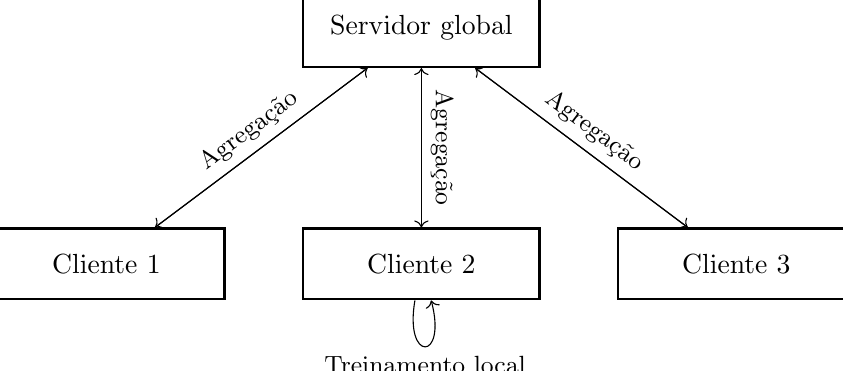
\begin{tikzpicture}[
    server/.style={rectangle, draw, thick, minimum width=3cm, minimum height=1cm, align=center},
    client/.style={rectangle, draw, thick, minimum width=3cm, minimum height=0.9cm, align=center},
    arrow/.style={->, thin}
]

\path[use as bounding box] (-5,-3) rectangle (5,1);

\node[server] (server) at (0,1)
{Servidor global};

\node[client] (c1) at (-4,-2) {Cliente 1};
\node[client] (c2) at (0,-2)  {Cliente 2};
\node[client] (c3) at (4,-2)  {Cliente 3};

\draw[arrow] (server) edge node[midway, above, sloped]{\small Agregação}  (c1);
\draw[arrow] (server) edge node[midway, above, sloped]{\small Agregação} (c2);
\draw[arrow] (server) edge node[midway, above, sloped]{\small Agregação}  (c3);

\draw[arrow] (c1) -- (server);
\draw[arrow] (c2) -- (server);
\draw[arrow] (c3) -- (server);

\draw[->, looseness=6, out=175, in=190]
(c1) edge node[left]{\small Treinamento local} (c1);

\draw[->, looseness=10, out=-100, in=-75]
(c2) edge node[below]{\small Treinamento local} (c2);

\draw[->, looseness=6, out=5, in=-10]
(c3) edge node[right]{\small Treinamento local} (c3);

\end{tikzpicture}
\caption{Fluxo básico do aprendizado federado.}\label{fig:federated_learning}
\end{figure}
\newpage\textbf{Diferenciação.} 
\begin{enumerate}
\item\textbf{Com relação à partição dos dados.} 
A classificação mais tradicional do federated learning diz respeito à forma como os dados estão distribuídos entre as entidades participantes. 
Conforme sistematizado por Zhang et al.~\cite{zhang2021survey}, 
essa categorização pode ser dividida em três cenários principais:
\begin{enumerate}
\item\textit{Aprendizado federado horizontal.}  
Nesse cenário, os conjuntos de dados possuem funcionalidades semelhantes, porém usuários distintos, 
isto é, há grande sobreposição no espaço de atributos, mas pouca interseção no espaço de instâncias. 
A partição ocorre ao longo das linhas da base de dados. 
Esse modelo é amplamente utilizado em aplicações como teclados inteligentes e sistemas de recomendação distribuídos, 
sendo o FedAvg~\cite{mcmahan2017communication} o algoritmo de agregação mais comum~\cite{zhang2021survey}.

\item\textit{Aprendizado federado vertical.}  
Aqui ocorre o oposto: os usuários são majoritariamente os mesmos, enquanto as funcionalidades são distintas. 
A partição é feita ao longo das colunas do conjunto de dados. 
Esse cenário é comum em colaborações interinstitucionais, como entre bancos e empresas de e-commerce, 
onde diferentes entidades possuem informações complementares sobre os mesmos usuários. 
Nesse contexto, técnicas baseadas em criptografia homomórfica e alinhamento seguro de entidades são amplamente utilizadas\cite{hardy2017private,cheng2021secureboost}.

\item\textit{Aprendizado federado com transferência.}  
Quando há pouca sobreposição tanto de usuários quanto de funcionalidades, 
recorre-se a técnicas de aprendizado por transferência para viabilizar o treinamento colaborativo. 
Esse modelo é particularmente útil em cenários com dados escassos ou rotulados de forma incompleta, 
como aplicações de classificação de imagem ou modelos de aprendizado de linguagem natural~\cite{yang2020}.
\end{enumerate}

\item\textbf{Com relação aos mecanismos de privacidade.} 
Embora o federated learning evite o compartilhamento direto dos dados brutos, 
a troca de parâmetros de modelo ainda pode levar ao vazamento de informações sensíveis. 
Dessa forma, diferentes mecanismos de privacidade são empregados:
\begin{enumerate}
\item\textit{Agregação segura de modelos.}  
Baseia-se na combinação de parâmetros locais sem que o servidor tenha acesso às atualizações individuais. 
Protocolos de \textit{secure aggregation} garantem que apenas o modelo global agregado seja observável~\cite{bonawitz2017practical}.

\item\textit{Criptografia homomórfica.}  
Permite que operações matemáticas sejam realizadas diretamente sobre dados criptografados, 
garantindo que nem o servidor nem outros participantes tenham acesso às informações originais. 
Esse método é comum em aprendizado federado vertical~\cite{hardy2017private,zhang2021survey}.

\item\textit{Privacidade diferencial.}
Consiste na adição controlada de ruído estatístico aos gradientes ou parâmetros do modelo, 
limitando a possibilidade de inferência sobre dados individuais. 
Pode ser aplicada tanto local quanto globalmente e é amplamente utilizada em sistemas reais, 
como os propostos e estudados pelo Google~\cite{mcmahan2018learning,bonawitz2019towards}.
\end{enumerate}

\item\textbf{Com relação ao modelo de aprendizado de máquina aplicado.} 
O federated learning não se restringe a um tipo específico de modelo, 
sendo aplicável a diferentes classes de algoritmos de aprendizado de máquina:
\begin{enumerate}
\item\textit{Modelos lineares.}  
Incluem regressão linear, regressão logística e ridge regression. 
Modelos lineares, como regressão linear e ridge regression, 
são frequentemente utilizados como ponto de partida em ambientes federados devido à sua simplicidade algorítmica e eficiência computacional, 
especialmente em cenários com restrições de privacidade e comunicação~\cite{nikolaenko2013privacy,zhang2021survey}.

\item\textit{Modelos baseados em árvores.}  
Árvores de decisão, random forests e gradient boosting têm sido adaptados para o contexto federado, 
especialmente em ambientes verticais. 
O SecureBoost é um exemplo representativo desse tipo de abordagem~\cite{cheng2021secureboost}.

\item\textit{Redes neurais profundas.}  
Redes neurais são amplamente utilizadas em aplicações modernas de federated learning, 
como reconhecimento de voz, visão computacional e sistemas embarcados. 
Frameworks baseados em FedAvg permitem o treinamento eficiente de redes profundas em larga escala~\cite{mcmahan2017communication,bonawitz2019towards}.
\end{enumerate}

\item\textbf{Com relação aos métodos de tratamento da heterogeneidade.} 
A heterogeneidade dos dados e dos recursos de clientes é um dos principais desafios inerente aos ambientes distribuídos,
que pode manifestar-se tanto na forma de dados estatisticamente 
não-IID\footnote{dados não-IID violam uma ou ambas dessas seguintes propriedades: independência e distribuição idêntica.
Assim, dados não-IID podem ser um sinal de que ou há viés no conjunto de dados, ou de que os dados não seguem a mesma distribuição,
ou de que há correlação local entre os dados. 
Uma vez que cada cliente coleta dados de acordo com comportamentos e contextos específicos,
resultando em distribuições distintas entre dispositivos, dados não-IID são um comum em aprendizado federado.}
quanto em diferenças computacionais,
de disponibilidade e de conectividade entre os dispositivos participantes.
Diversos mecanismos têm sido propostos na literatura para mitigar esses efeitos adversos:
\begin{enumerate}
\item\textit{Comunicação assíncrona.}
Abordagens assíncronas permitem que o servidor agregue atualizações de clientes à medida que elas se tornam disponíveis,
sem a necessidade de sincronização global entre todos os participantes.
Esse modelo reduz o impacto de \textit{stragglers} e dispositivos com conectividade intermitente,
sendo particularmente adequado para cenários em larga escala e ambientes móveis~\cite{zhang2021survey}.

\item\textit{Amostragem de clientes.}
Em sistemas federados reais, apenas um subconjunto dos clientes disponíveis participa de cada rodada de treinamento.
A amostragem de clientes reduz significativamente os custos de comunicação e computação,
além de tornar o processo mais robusto à heterogeneidade de recursos.
Esse mecanismo é parte fundamental do algoritmo FedAvg e de seus desdobramentos~\cite{mcmahan2017communication}.

\item\textit{Mecanismos tolerantes a falhas.}  
Falhas de comunicação, desconexões inesperadas e clientes lentos são comuns em ambientes federados.
Métodos tolerantes a falhas buscam garantir a continuidade do treinamento e preservar propriedades de convergência
mesmo na presença de clientes ausentes ou atualizações perdidas.
Embora fora do escopo do aprendizado federado supervisionado tradicional,
trabalhos em Federated Reinforcement Learning (FRL), como o de Fan et al.~\cite{fan2022fault},
formalizam esse problema e propõem estratégias que mantêm a estabilidade do treinamento
sob diferentes modelos de falha.

\item\textit{Heterogeneidade de modelos e aprendizado personalizado.}  
Para lidar com distribuições de dados altamente não-IID, abordagens de aprendizado federado personalizado
permitem a coexistência de modelos locais adaptados a cada cliente juntamente com um modelo global compartilhado.
O trabalho de Liang et al.~\cite{liang2020think} propõe a separação entre representações globais e locais,
reduzindo o impacto da heterogeneidade estatística e melhorando o desempenho individual dos clientes.
\end{enumerate}
\end{enumerate}
\section{Desafios}

% ---- Bibliography ----
%
% BibTeX users should specify bibliography style 'splncs04'.
% References will then be sorted and formatted in the correct style.
%
\bibliographystyle{splncs04}
\bibliography{refs}
%
\end{document}
